\vspace{-1.em}
\section{Introduction}

Diffusion models~\cite{diffusion,ddpm,scoresde} and their flow-based variants~\cite{fm,rectified,stochasticflow} are highly effective for generative modeling.
These models can be viewed as solving a differential equation (\eg an ODE) that maps a prior distribution to the data distribution.
Because these equations are typically solved using multi-step numerical solvers, the generation process requires a certain number of function evaluations (NFEs).

Recently, encouraging progress~\cite{cm,ict,ect,scm,shortcut,imm,mf} has been made toward reducing sampling steps in diffusion/flow-based models.
Using the concept from physical simulation, these models can be thought of as \emph{fastforward} approximations to the underlying differential equations.
The resulting fastforward models are capable of generating in a very few or even one step.
To achieve this goal, the training objectives are formulated as look-ahead mappings that operate across large time intervals, and various approximations have been proposed to address this challenging problem.

\begin{figure}
    \centering
    \vspace{-1em}
    \begin{subfigure}[t]{0.35\linewidth}
        \centering
        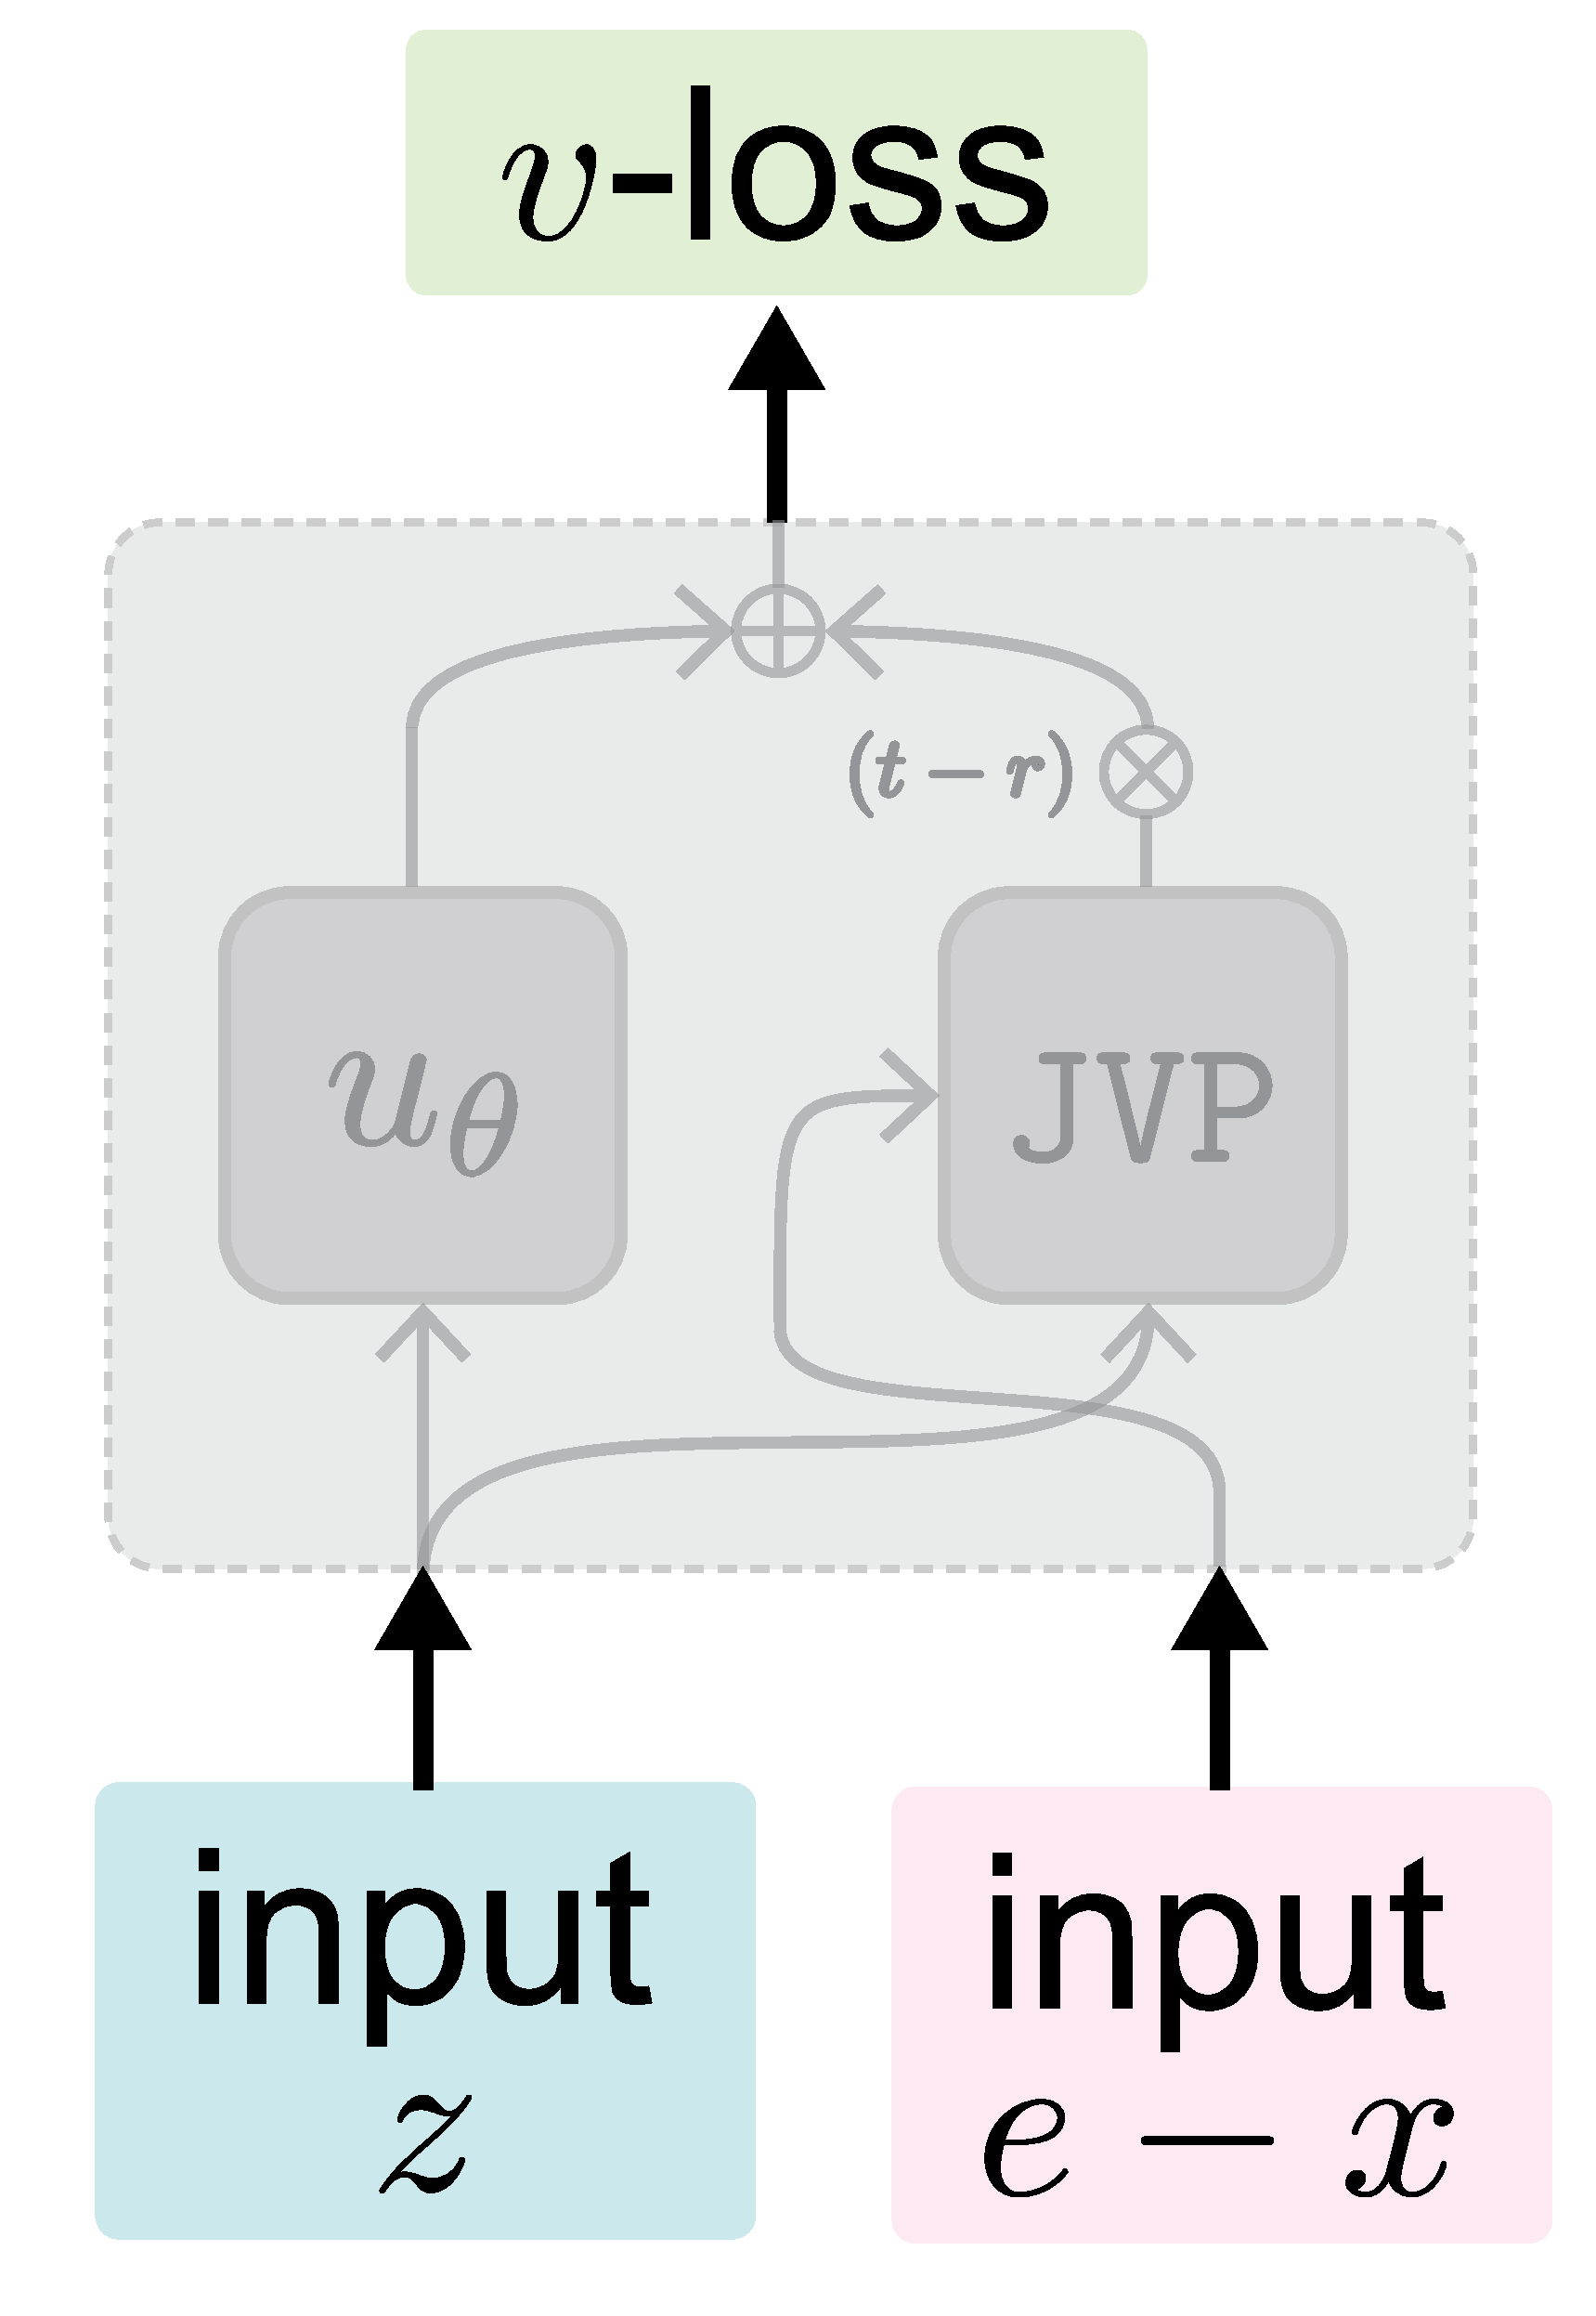
\includegraphics[width=\linewidth,clip,page=1]{figs/teaser.pdf}
        \caption{\centering Original MeanFlow}
        \label{fig:teaser_mf}
    \end{subfigure}
    \hspace{0.1\linewidth}
    \begin{subfigure}[t]{0.35\linewidth}
        \centering
        \includegraphics[width=\linewidth,clip,page=2]{figs/teaser.pdf}
        \caption{\centering Improved MeanFlow}
        \label{fig:teaser_imf}
    \end{subfigure}
    \vspace{-.2em}
    \caption{
    \textbf{Conceptual comparison}. Original MeanFlow (MF) \cite{mf} predicts \textit{average velocity} $u$ by a network $u_\theta$. As the ground-truth $u$ is unknown, original MF substitutes $u$ with the network's own prediction. We show that the original MF objective is equivalent to a loss on the \textit{instantaneous velocity} $v$ (namely, $v$-loss), but re-parameterized by the neural network $u_\theta$ (namely, $u$-pred), as shown in \textbf{(a)}. This re-parameterization, encompassed within the gray box, is determined by \textit{the MeanFlow identity} \cite{mf}.
    This reformulation reveals that the input to the compound function (in the gray box) is not only the noisy data (here, $z$), but also the conditional velocity ($e - x$), which is not a standard regression problem. In \textbf{(b)}, our improved objective is conceptually \emph{\textbf{$v$-loss re-parameterized by $u$-pred}}, taking only the legitimate input $z$.
    }
    \vspace{-.7em}
    \label{fig:teaser}
\end{figure}

In this work, we take a deeper look at the recently proposed MeanFlow (MF) framework~\cite{mf}.
In MF, instead of learning the \emph{instantaneous velocity} field (denoted by $v$) underlying the ODE, the model learns an \emph{average velocity} field (denoted by $u$) across time steps. 
To avoid infeasible integration during training, MF reformulates the problem into a differential relation between the instantaneous and average velocity fields.
This relation, called the ``MeanFlow identity''~\cite{mf}, establishes a trainable objective.  
The underlying average velocity field serves as the ground-truth and as the optimum of this training objective.

Despite the encouraging results of the original MF~\cite{mf}, we identify two major issues that remain unresolved: (i) the training target in the original MF is network-dependent and therefore does not constitute a standard regression problem; (ii) MF handles the classifier-free guidance (CFG) \cite{cfg} using a fixed training-time guidance scale, which sacrifices flexibility. 
We analyze these issues and present our solutions.

First, the original MF predicts the average velocity $u$, an unknown quantity that is substituted with the network's own prediction $u_\theta$. To have a network-agnostic prediction target, we show that the original MF can be equivalently reformulated as a loss on the instantaneous velocity (namely, $v$-loss), which is \textit{re-parameterized} by the network that predicts the average velocity $u$ (namely, $u$-pred). See \cref{fig:teaser}\textbf{(a)}. 
This reformulation provides a regression target $v$ that does not depend on the network.
From this perspective, we further propose to reformulate the regression input, enforcing it to depend only on the noisy sample but not on other unknown quantities (\cref{fig:teaser}\textbf{(b)}). Our improved objective substantially stabilizes the training process in practice.

Second, the original MF handles CFG \cite{cfg} using a \textit{fixed} guidance scale that is determined before training. We suggest that fixing the guidance compromises the flexibility at inference time, and that the optimal value depends on the model’s capability. To address this, we reformulate the guidance as a form of \textit{conditioning}, allowing it to take varying values during both training and inference. This formulation unlocks the power and flexibility of CFG while still maintaining the 1-NFE sampling behavior.
We further design an improved architecture that accommodates this and other types of conditions through in-context conditioning.

Overall, our experiments show that our \textbf{improved MeanFlow} (\textbf{iMF}) effectively addresses these issues in the original MF. In the challenging setting of 1-NFE generation on ImageNet 256$\times$256 trained from scratch, iMF achieves an FID of \textbf{1.72}, representing a relative 50\% improvement over the original MF and setting a new state-of-the-art of its kind.
Our models do not use distillation or any pre-trained models for alignment. 
This result substantially narrows the gap with those of multi-step methods, suggesting that fastforward generative models can be a promising stand-alone framework.
